% !TeX encoding = UTF-8
\section{Safety of multigram}
Let's introduce some reducible multigrams: A \textit{tetragram} is a sequence ($v_1$, $v_2$, $v_3$, $v_4$) of vertices of $G$ such that it can build a facial cycle in this listed order. Analogously, we can define a \textit{hexagram} ($v_1$, $v_2$, $v_3$, $v_4$, $v_5$, $v_6$). And a \textit{pentagram} ($v_1$, $v_2$, $v_3$, $v_4$, $v_5$) is also defined likewise but with the limitation: $v_1$, $v_2$, $v_3$, $v_4$ have degree exactly three.

\subsection{Safe multigrams}
As was pointed out in the last section to this paper, the detected multigrams should possess some attributions, which is called \textit{safety}. Assume that $k$ = 4, 5, 6 and ($v_1, v_2, ..., v_k$) be a tetra-, penta- or hexagram in a triangle-free planar graph $G$. On the occasion that $k$ = 4 or $k$ = 6, the tetragram or hexagram is $safe$ if every path in $G$ of length at most three with ends $v_1$ and $v_3$ is a subgraph of cycle $v_1v_2...v_k$, which means the path(s) from $v_1$ to $v_3$ of length at most three has to be part of multigrams. The safety of pentagram is bit complicated: let $x_i$ be the neighbor of $v_i$ different from $v_{i-1}$ and $v_{i+1}$, where $v_0 = v_5$. Thus $x_i \notin$ \{$v_1, v_2, v_3, v_4, v_5$\} for the reason that if that is the case, the vertices $v_i$, $x_i$ form a triangle with $v_{i-1}$ or $v_{i+1}$, which is a contradiction to the triangle-free graph. A pentagram ($v_1, v_2, v_3, v_4, v_5$) is \textit{safe} \cite{dvorak2013threecoloring}, if
\begin{itemize}
    \item the vertices $x_1, x_2, x_3, x_4$ are pairwise distinct and pairwise non-adjacent, and
    \item there is no path in $G \backslash \{v_1, v_2, v_3, v_4\}$ of length at most three from $x_2$ to $v_5$, and
    \item every path in $G \backslash \{v_1, v_2, v_3, v_4\}$ of length at most three from $x_3$ to $x_4$ has length exactly two, and its completion via the path $x_3v_3v_4x_4$ results in a facial cycle of length five in $G$.
\end{itemize}

\begin{definition}
Given a facial cycle $C$ of length four, \textit{identifying a pair of
diagonally opposite vertices of $C$} means that the two selected vertices $u, v \in V(C)$ will be "glued" as a vertex. It results $|V(C^{'})| = |V(C)| - 1$.
\end{definition}

\subsection{Identifying vertices and reconstruction of graph}

If there exists a safe tetra- or hexagram, $G^{'}$ can be obtained by identifying vertices $v_1$ with $v_3$. $v_1$ in \textbf{Figure 6, 7} is at the same time $v_3$ as well. For \textit{tetragram} $(v_1, v_2, v_3, v_4)$:
\begin{figure}[H] %H为当前位置,!htb为忽略美学标准,htbp为浮动图形
\centering %图片居中
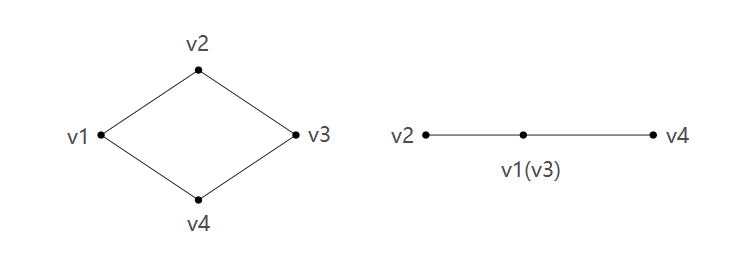
\includegraphics[width=0.6\textwidth]{figure/identifyingv1v3.png} 
\label{figure} %用于文内引用的标签
\caption{Identifying $v_1$ and $v_3$ in a safe tetragram}
\end{figure}

\textit{Reconstruction step: }In graph $G^{'}$, we can assign colors as follows: let $c_1$ be the color of $v_2$, $c_2$ be the color of $v_1$ and $c_3$ be the color of $v_4$. Clearly that we can also color $v_3$ with $c_2$, since $v_1$ and $v_3$ are not adjacent and the tetragram is safe.\\

For \textit{hexagram} $(v_1, v_2, v_3, v_4, v_5, v_6)$: 
\begin{figure}[H] %H为当前位置,!htb为忽略美学标准,htbp为浮动图形
\centering %图片居中
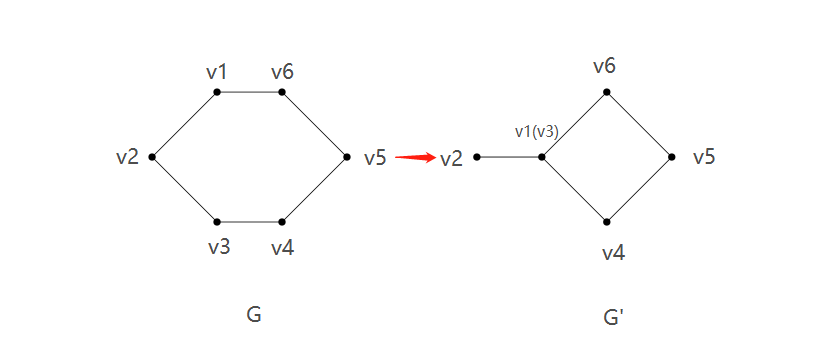
\includegraphics[width=0.7\textwidth]{figure/identifyingv1v32.png} 
\label{figure} %用于文内引用的标签
\caption{Identifying $v_1$ and $v_3$ in a safe pentagram}
\end{figure}

\textit{Reconstruction step: }In graph $G^{'}$, we can assign colors following these principles: let $c_1$ be the color of $v_2$, $c_2$ be the color of $v_1$. We can determine colors of $v_4$ and $v_6$ arbitrarily. Assume that the color of $v_4$ and $v_6$ is $c_3$ and the color of $v_5$ is $c_1$. Apparently, the color can be designated for $c_2$ as well, since $v_1$ and $v_3$ are not adjacent and the hexagram is safe.\\

The case of pentagram ($v_1$, $v_2$, $v_3$, $v_4$, $v_5$) is significantly different. $G^{'}$ will be attained from $G \backslash \{v_1, v_2, v_3, v_4\}$ by identifying $v_5$ with $x_2$ and $x_3$ with $x_4$.

\begin{figure}[htbp]
\centering
\begin{minipage}[t]{0.48\textwidth}
\centering
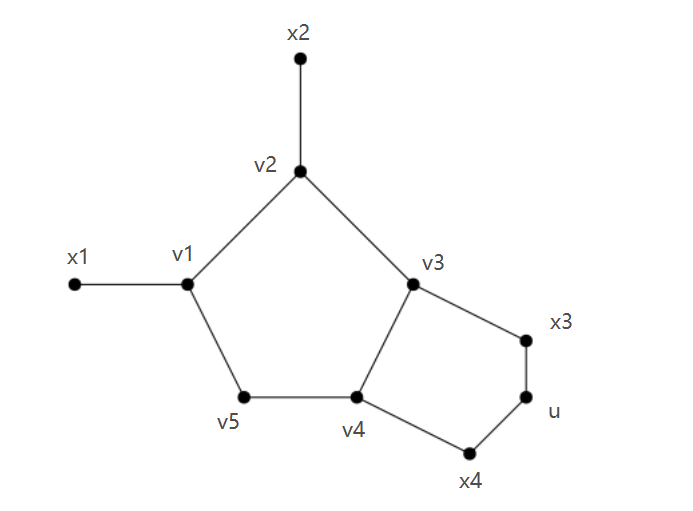
\includegraphics[width=1\textwidth]{figure/pentagram.png}
\caption{$G$}
\end{minipage}
\begin{minipage}[t]{0.48\textwidth}
\centering
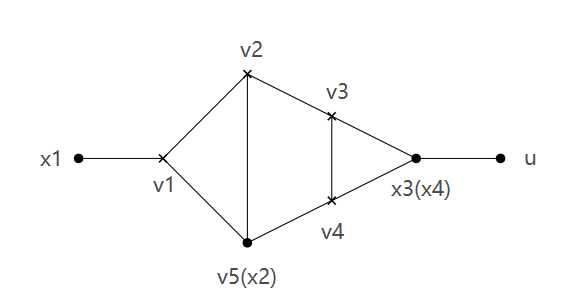
\includegraphics[width=1\textwidth]{figure/pentagram_prime.png}
\caption{$G^{'}$}
\end{minipage}
\end{figure}

\textit{Reconstruction step: }In graph $G^{'}$, let $c_1$ be the color of $x_1$, $c_2$ the color of $x_2$ and $v_5$, and $c_3$ the color of $x_3$ and $x_4$. Consider the following cases:
\begin{itemize}
    \item $c_1 = c_2$, we will color the remaining vertices in this order ($v_4, v_3, v_2, v_1$). Since there are at most two remaining colors when $v_i$ is colored, we can simply choose the third color for it. 
    \item $c_2 = c_3$, similarly, we will color the vertices in the reversed order as in the first case.
    \item $c_1 \ne c_2 \ne c_3$, we can color $v_2$ with $c_1$, $v_1$ with $c_3$, $v_3$ with $c_2$ and $v_4$ with $c_1$.
\end{itemize}

\subsection{Counterexamples: unsafe multigrams}
Subsequently, let's take care of the importance of multigrams. What happens, when we identify certain pair of vertices if the given multigrams are not safe? If a tetragram or hexagram is not safe, then there exists a path of length at most three that is not part of tetragram or hexagram.
\begin{figure}[H] %H为当前位置,!htb为忽略美学标准,htbp为浮动图形
\centering %图片居中
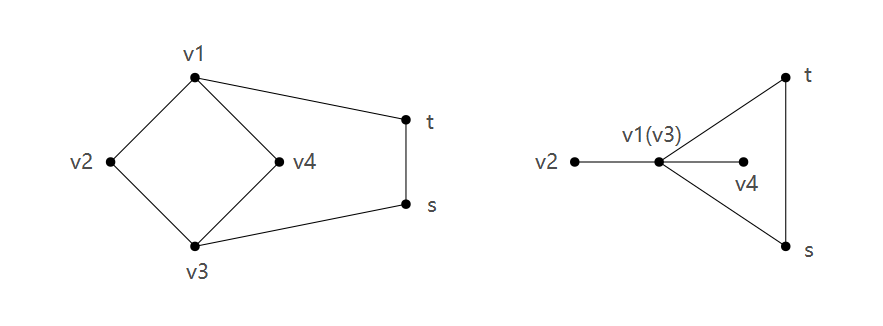
\includegraphics[width=0.7\textwidth]{figure/unsafetetragram.png} 
\caption{An unsafe tetragram} %最终文档中希望显示的图片标题
\label{figure} %用于文内引用的标签
\end{figure}

\begin{figure}[H] %H为当前位置,!htb为忽略美学标准,htbp为浮动图形
\centering %图片居中
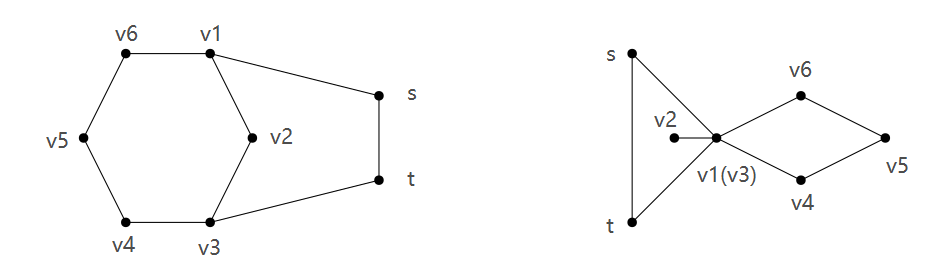
\includegraphics[width=0.7\textwidth]{figure/unsafehexagram.png} 
\caption{An unsafe hexagram} %最终文档中希望显示的图片标题
\label{figure} %用于文内引用的标签
\end{figure}
Observed from above figures that after identifying vertices $v_1$ with $v_3$, a triangle consisting of $s, t, v_1$ will be created.\newline \\
If a pentagram is not safe, then it has either a path in $G \backslash \{v_1, v_2, v_3, v_4\}$ at most three from $x_2$ to $v_5$ or a path in $G \backslash \{v_1, v_2, v_3, v_4\}$ from $x_3$ to $x_4$ of length 3.
\begin{figure}[H] %H为当前位置,!htb为忽略美学标准,htbp为浮动图形
\centering %图片居中
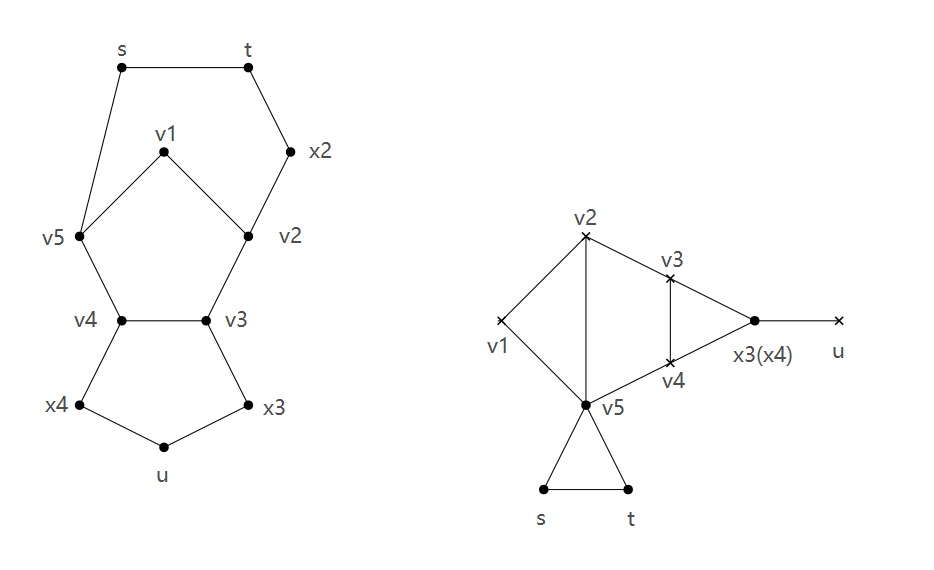
\includegraphics[width=0.7\textwidth]{figure/Inkedunsafepentagram1_LI.jpg} 
\label{figure} %用于文内引用的标签
\caption{Unsafe pentagram, case 1}
\end{figure}

\begin{figure}[H] %H为当前位置,!htb为忽略美学标准,htbp为浮动图形
\centering %图片居中
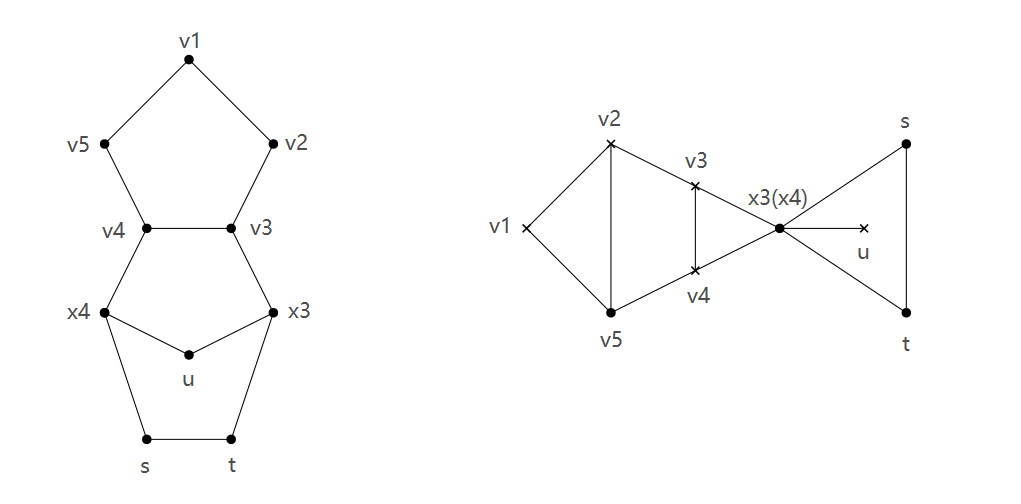
\includegraphics[width=0.7\textwidth]{figure/unsafepentagram2.png} 
\label{figure} %用于文内引用的标签
\caption{Unsafe pentagram, case 2}
\end{figure}
Noticed that in the former case, $v_5$($x_2$), $s$ and $t$ build a triangle and in the latter case, $x_3$($x_4$), $s$ and $t$ build a triangle in the same way.

%----------------------------------------------------------------------
\section{Proof of Grötzsch's theorem}
Firstly, we introduce a method that is often used in graph theory. 
\textit{Discharging method} is a technique used to prove lemmas in structural graph theory. Initially, a charge is assigned to each face and each vertex of the graph. The charges are assigned so that they sum to a small positive number. During the Discharging Phase the charge at each face or vertex may be redistributed to nearby faces and vertices. However, each discharging rule maintains the sum of the charges. \cite{discharging}

\begin{observation}
\begin{align*}
    \sum_{f \in F}deg(f) = 2|E| \ and \ \sum_{v \in V}deg(v) = 2|E|
\end{align*}
%$\sum_{f \in F}deg(f) = 2|E|$ and $\sum_{v \in V}deg(v) = 2|E|$.
\end{observation}

\begin{theorem}[Euler's formula]
If a finite, connected, planar graph is drawn in the plane without any edge intersections, and $v$ is the number of vertices, $e$ is the number of edges and $f$ is the number of faces (regions bounded by edges, including the outer, infinitely large region), then: $v-e+f=2$. \cite{euler}
\end{theorem}

\begin{proof}
By induction on the number of edges $e$.\\
\textit{Base case: } Show that the statement holds for the smallest natural number $e$ = 0.\\
$e$ = 0, $v$ = 1, $f$ = 1 \ $\xrightarrow{}$ 1 - 0 + 1 = 2. \\
\\
\textit{Inductive step: }Show that for any e $\geq$ 0, if $e = n$ holds, then $e = n + 1$ holds as well. \\
\textit{Case 1: }$G$ is a tree. It follows $v = e + 1 = n + 2$, $f = 1$. $\longrightarrow$ $v - e + f = (n + 2) - (n+1) + 1 = 2$.\\
\textit{Case 2: }There exists a simple cycle. Assume that there is a spanning tree $T$. $(u, v)$ is an edge which does not belong to $T$. The path between $u$ and $v$ builds a simple cycle with the edge $uv$. Removal of the edge $uv$ constructs a connect graph $G^{'}$ with $v^{'}$ $ = v$, $e^{'}$ $=e - 1$ and $f^{'}$ $= f - 1$. \\
It leads from induction hypothesis that 2 = $v^{'}$ - $e^{'}$ + $f^{'}$ = $v + (e - 1) + (f - 1) = v - e + f$.\
\end{proof}

\begin{lemma}
Let $G$ be a connected triangle-free plane graph and let $f_0$ be the
unbounded face of $G$. Assume that the boundary of $f_0$ is a cycle $C$ of length
at most six, and that every vertex of $G$ not on $C$ has degree at least three. If
$G \ne C$, then $G$ has either a tetragram, or a pentagram ($v_1, v_2, v_3, v_4, v_5$) such
that $v_1, v_2, v_3, v_4$ $\notin V(C)$. \cite{dvorak2013threecoloring}
\end{lemma}

\begin{proof}
Assign the charge of a vertex $v$ to be 3deg($v$) - 12, the charge of the face $f_0$ to be $3|V(C)|$ + 11 and the charge of a face $f \ne f_0$ of length $\ell$ to be $3 \ell - 12$. 
    \begin{claim}
    The sum of the charges of all vertices and faces is -1.
    \end{claim}
    \begin{proof}
        \begin{align*}
            & Sum \ of \ charges \ = \sum_{v \in V}(3deg(v) - 12) + \sum_{f \in F \backslash {f_0}} (3\ell - 12) + 3|V(C)| + 11 \\
            &= \underbrace{3 \cdot 2|E| - 12 |V| + 3\cdot2|E| - 12|F|}_{\text{apply Euler's formula here: v + f - e = -2}} - (3\ell_{f_0} - 12) + 3|V(C)| + 11 \\
            &=-2 \cdot 12 + 3|V(C)|- 3\ell_{f_0} + 12 + 11\\
            &= -1
        \end{align*}
    \end{proof}
    Afterwards, we redistribute the charges conforming to the following rules:
    \begin{itemize}
        \item[(1)] Every vertex $v \notin C$ and deg($v$) = 3 will receive one unit of charge from each incident face.
        \item[(2)] Every vertex $v \in C$ and deg($v$) = 3 will receive three units from $f_0$.
        \item[(3)] Every vertex $v \in C$ and deg($v$) = 2 will receive five units from $f_0$ and one unit from the other incident face. 
    \end{itemize}
    
    \begin{claim}
    The final charge of $f_0$ is non-negative.
    \end{claim}
    
\begin{proof}
Let $\ell$ be the size of cycle $C$. As we defined above, the initial charge of face $f_0$ is $3 \ell + 11$. According to \textbf{Lemma 4.2}($G \ne C$), we know that there is at least one vertex on $C$ whose degree is at least three, which leads that there are at most $(\ell - 1)$ vertices of $C$ with degree two and one vertex on $C$ has degree at least three. Thus, $f_0$ can send at most obeying rules (2) and (3) $\big(5(\ell - 1) + 3\big)$ units of charge.\\
$\longrightarrow$ The final charge of $f_0$ = $3\ell + 11 - 5(\ell - 1) - 3 = 13 - 2\ell \geq 1$, since the length of the outer face is at most six.
\end{proof}
Noticed that among above three rules, all vertices do not send any units of charge. Hence, the charge of all vertices is also non-negative. In consonance with the definition of discharging method, the total sum before and after charging should keep unchanged, which contributes to the existence of a face $f \ne f_0$ whose final charge is strictly negative. From rule (1) informed that $f$ will send at most one unit to each incident vertex. The final charge is $3\ell - 12 - \ell = 2\ell - 12$, which is, as discussed, smaller than 0. It follows that the length of $f$ is at most five. Moreover, if $f$ has length exactly five, its initial charge is $3\ell - 12 = 3$, then $f$ has to have at least four incident vertices. And all these vertices cannot be on $C$ and have degree two. Otherwise, $f$ will send nothing to the ends of the common subpath of $f$ and $f_0$. As a deduction, the vertices of $f$ structure a tetragram or a pentagram.
\end{proof}

\begin{lemma}
Every triangle-free plane graph $G$ of minimum degree at least three has a safe tetragram, a safe pentagram or a safe hexagram. \cite{dvorak2013threecoloring}
\end{lemma}
\begin{proof}
Let $G$ as stated. 

\begin{claim}
Suppose that $(v_1, v_2, v_3, v_4)$ is a tetragram in $G$ which bounds a face, then one of tetragrams $(v_1, v_2, v_3, v_4)$, $(v_2, v_3, v_4, v_1)$ is safe.
\end{claim}

\begin{proof}
Prove by contradiction: assume that both of tetragrams are unsafe, which implies that there is no pair of diagonally opposite vertices.
\begin{itemize}
    \item[(1)] \textit{\textbf{$v_1$ and $v_3$ is not the pair diagonally opposite vertices.}} So there is a path from $v_1$ to $v_3$ that is not part of graph $G$ of length at three. See the case in \textbf{Figure 14}.
    \item[(2)] \textit{\textbf{$v_2$ and $v_4$ is not the pair diagonally opposite vertices.}} Then there must exist a path from $v_2$ to $v_4$ of length at most three. 
    \begin{figure}[H] %H为当前位置,!htb为忽略美学标准,htbp为浮动图形
    \centering %图片居中
    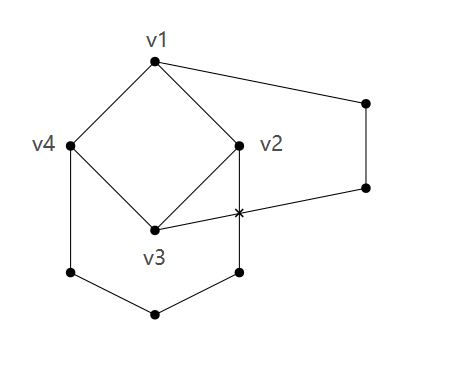
\includegraphics[width=0.4\textwidth]{figure/4face.png} 
    \label{figure} %用于文内引用的标签
    \caption{4-face ($v_1, v_2, v_3, v_4$)}
    \end{figure}
    Since the tetragram ($v_1, v_2, v_3, v_4$) is a 4-face, the path has to be outside of the face, which results that there is a cross among two paths which is a contradiction to the planarity.
\end{itemize}
\end{proof}
Therefore, we may assume that $G$ has no 4-face. It follows that every 4-cycle is separating. If $G$ features a separating cycle of length at the most five, then select the separating cycle $C_1$ in order that the bounded disk is smallest possible and let $G_1$ be the subgraph of $G$ consisting of all vertices and edges drawn in the closed disk bounded by $C_1$. If $G$ has no separating cycle of length at most five, then let $G_1 := G$ and let $C_1$ be a facial cycle of $G$ of length at the most five. In addition, we reform the $G$ that $C_1$ is the outer face.

\begin{lemma}
The minimum degree of $G$ is at least three, then there exists a facial cycle $C_1$ of $G$ of length at most five.
\end{lemma}

\begin{proof}
By contradiction, assume there is no face of length at
most 5, which means every face has length at least 6. In this case, we have every vertex degree at least 3, so we have $e \geq \frac{3}{2} \cdot v$ $\Longleftrightarrow$ $v \leq \frac{2}{3} \cdot e$ in view of the fact that each vertex contributes at least 3 edges, but we have counted each edge twice, so have to divide by 2. Similarly, since every face is of length at least 6, so $e \geq \frac{6}{2} \cdot f$ $\Longleftrightarrow$ $f \leq \frac{1}{3} \cdot e$. Supposing that we plug these into Euler's formula, we get:
\begin{equation*}
    2 = v + f - e \leq \frac{2}{3}e + \frac{1}{3}e - e = 0
\end{equation*}
This is a contradiction.
\end{proof}

Observed that no separating cycle of length at most five can be contained in $G_1$ for the reason that otherwise we can choose that smaller cycle to be $C_1$. Hence, there is no 4-cycle in $G_1$ except possibly $C_1$, because 
\begin{itemize}
    \item it cannot be a 4-face, as proved in \textbf{Claim 4},
    \item there is no 4-separating cycle as mentioned.
\end{itemize}
A step further, we can define a subgraph $G_2$ of $G_1$ and the facial cycle $C_2$ of $G_2$ in this way: If there is a separating cycle of length six in $G_2$, then assign $C_2$ to be the cycle in which fewest vertices and edges are contained. $G_2$ is then the subgraph of all vertices and edges in which the cycle $C_2$ bounds. As analog to the case of $G_1$, there is no separating cycle of length at most six in $G_2$. Meanwhile, we've assumed that no 4-face is permitted, it leads that every cycle of length at most six in $G_2$ bounds a face. What's more, $C_2$ is a induced cycle from $G_2$. If it would not be the case, namely there would be a chord inside $C_2$, we could then choose a smaller cycle, which is a contradiction to the minimality. 

We can apply \textbf{Lemma 4.2.} on graph $G_2$ and the facial cycle $C_2$ and conclude that $G_2$ has a pentagram ($v_1, v_2, v_3, v_4, v_5$) with $v_1, v_2, v_3, v_4 \notin V(C_2)$.
\begin{itemize}
    \item[(1)] \textit{\textbf{At least one of pentagrams ($v_1, v_2, v_3, v_4, v_5$) and ($v_4, v_3, v_2, v_1, v_5$) is safe.}} Then the lemma holds.
    \item[(2)] \textit{\textbf{None of them is safe.}} $\forall i \in \{1, 2, 3, 4\}$, let $x_i$ be the neighbor of $v_i$ other than $v_{i-1}$ and $v_{i+1}$, where $v_0 = v_5$. Noticed that $x_1, x_2, x_3, x_4$ belong to $G_2$ because otherwise it might create crosses between the incident edges with neighbors and $C_2$, and they are pairwise distinct and non-adjacent, since 
    \begin{itemize}
        \item $G_2$ is triangle-free,
        \item no separating cycle at most 5,
        \item no 4-cycle except $C_2$.
    \end{itemize}
    It results $|\{x_1, x_2, x_3, x_4\} \cap V(C_2)| \leq 3$.
    \begin{figure}[H] %H为当前位置,!htb为忽略美学标准,htbp为浮动图形
    \centering %图片居中
    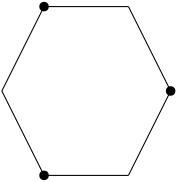
\includegraphics[width=0.2\textwidth]{figure/intersect3vertices.png} 
    \caption{The number of intersection $\leq$ 3} %最终文档中希望显示的图片标题
    \label{figure} %用于文内引用的标签
    \end{figure}
    If the number of intersection among these above two sets would be 4, then two of them have to be adjacent, which is a contradiction.

\begin{lemma}
If $v_5 \in V(C_2)$, then $\{x_1, x_2, x_3, x_4\} \cap V(C_2) = \emptyset$.
\end{lemma}
\begin{proof}
We assume that at least one of $x_3$ and $x_4$ is not on $C_2$.
\begin{itemize}
    \item[Case 1:] \textit{\textit{$x_4$ is not on $C_2$.}} Suppose that $x_3$ lies on $C_2$. \begin{figure}[H] %H为当前位置,!htb为忽略美学标准,htbp为浮动图形
    \centering %图片居中
    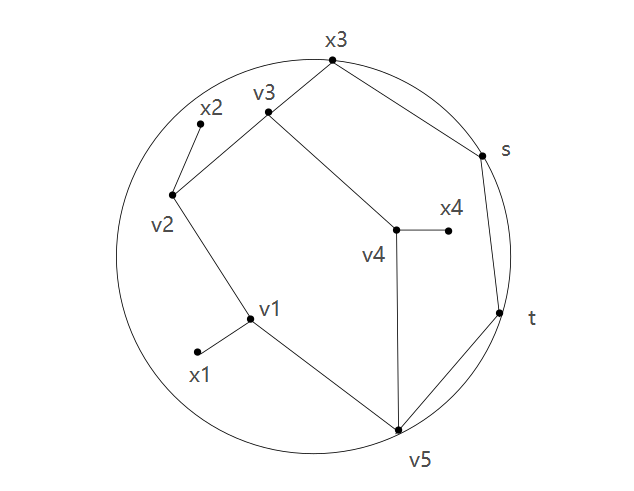
\includegraphics[width=0.6\textwidth]{figure/x4notonc2.png} 
    \caption{$x_4$ not on $C_2$, $x_3$ on $C_2$} %最终文档中希望显示的图片标题
    \label{figure} %用于文内引用的标签
    \end{figure}
    It leads to a contradiction to the minimality of cycle $C_2$, for the reason that there is a smaller 4-separating cycle $x_3v_3v_4v_5$ or 5-separating cycle $x_3v_3v_4v_5s$ or 6-separating cycle $x_3v_3v_4v_5st$ containing $x_4$. Observed that if $x_2$ lies on $C_2$, it's analog to the former case when $x_3$ is on $C_2$. May assume now that $x_1$ lies on $C_2$:
    \begin{figure}[H] %H为当前位置,!htb为忽略美学标准,htbp为浮动图形
    \centering %图片居中
    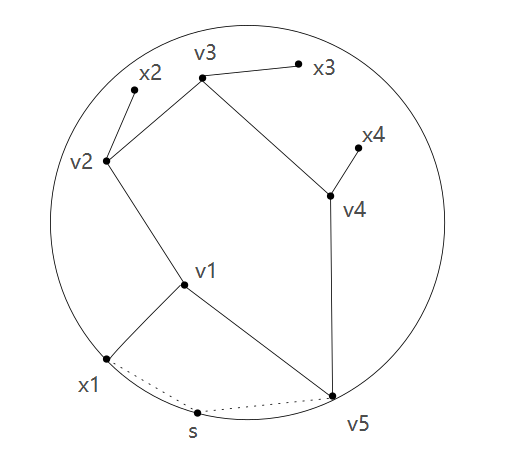
\includegraphics[width=0.5\textwidth]{figure/x1notonc2.png} 
    \caption{$x_4$ not on $C_2$, $x_1$ on $C_2$} %最终文档中希望显示的图片标题
    \label{figure} %用于文内引用的标签
    \end{figure}
    It results also a contradiction to the minimality of $C_2$, because it's required to have at least one extra vertex on $C_2$ between $x_1$ and $v_5$, since no triangle in planar graph is permitted. In consequence, we find a smaller separating cycle which just visits $v_1$ with path $x_1sv_5$ instead of visiting $s$ with path $x_1v_1v_5$.
    \item[Case 2:] \textit{\textit{$x_3$ is not on $C_2$.}} We may assume that $x_4$ is on $C_2$, otherwise it belongs to case 1. 
    \begin{figure}[H] %H为当前位置,!htb为忽略美学标准,htbp为浮动图形
    \centering %图片居中
    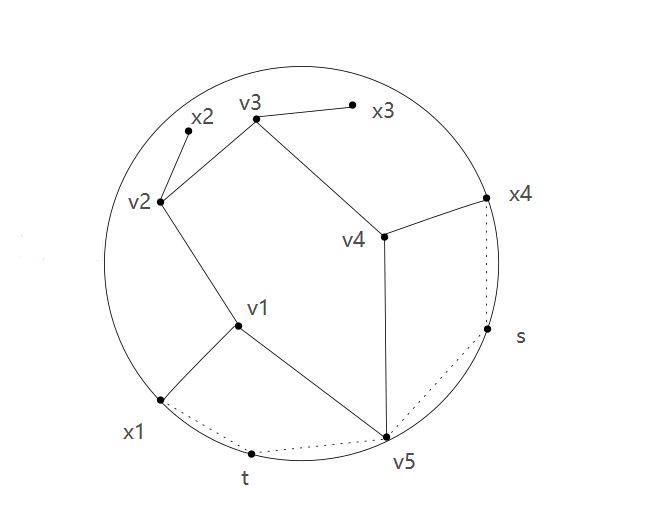
\includegraphics[width=0.6\textwidth]{figure/x3notonc2.png} 
    \caption{$x_3$ not on $C_2$, $x_1$ on $C_2$} %最终文档中希望显示的图片标题
    \label{figure} %用于文内引用的标签
    \end{figure}
    All cases under this circumstance are totally similar to the case 1.
\end{itemize}
\end{proof}

\end{itemize}
Since the pentagram ($v_1, v_2, v_3, v_4, v_5$) is not safe, we know that, according to the definition of safety, there exists a pair of vertices $x$ and $y$ so that $\{x, y\} = \{x_3, x_4\}$ or $\{x, y\} = \{x_2, v_5\}$ and a path $P$ in $G \backslash \{v_1, v_2, v_3, v_4\}$ of length at most three ended with $x$ and $y$, which either 
\begin{itemize}
    \item is from $x_2$ to $v_5$, or
    \item has length exactly three from $x_3$ to $x_4$ or its completion via the path $x_3v_3v_4x_4$ doesn't result in a facial cycle of length five in $G$.
\end{itemize}
If $\{x, y\} = \{x_3, x_4\}$, let $Q$ be the path $x_3v_3v_4x_4$; otherwise $x_2v_2v_1v_5$. Then we have following cases:
\begin{itemize}
    \item[Case 1:] \textit{\textbf{$P \cup Q$ bounds a facial cycle in $G$.}} Thus, we know that $\{x, y\} = \{x_3, x_4\}$ and the length of path $P$ is exactly three. Suppose $P \cup Q$ is listed in this order $x_3v_3v_4x_4ab$.
    \begin{claim}
    $(x_4, v_4, v_3, x_3, a, b)$ is a safe hexagram. 
    \end{claim}
    \begin{proof}
    By contradiction: there would be a path from $x_4$ to $v_3$ of length at most three that is not part of this hexagram. Assume that this path would be $x_4u_1v_3$ or $x_4u_1u_2v_3$, where $u_1, u_2 \ne v_4$.
    \begin{itemize}
        \item \textit{\textbf{The path is $x_4u_1v_3$.}} Noted that $v_3$ has degree exactly three according to the definition of pentagram and its neighbors are $v_2$, $v_4, x_3$. In addition, $v_2$ has also degree exactly three and has neighbors $v_1, x_2, v_3$. So $u_1$ can't be $v_2$. What's more, $x_3, x_4$ are non-adjacent. It follows that this case is not possible.
        \item \textit{\textbf{The path is $x_4u_1u_2v_3$.}} 
        \begin{figure}[H] %H为当前位置,!htb为忽略美学标准,htbp为浮动图形
            \centering %图片居中
            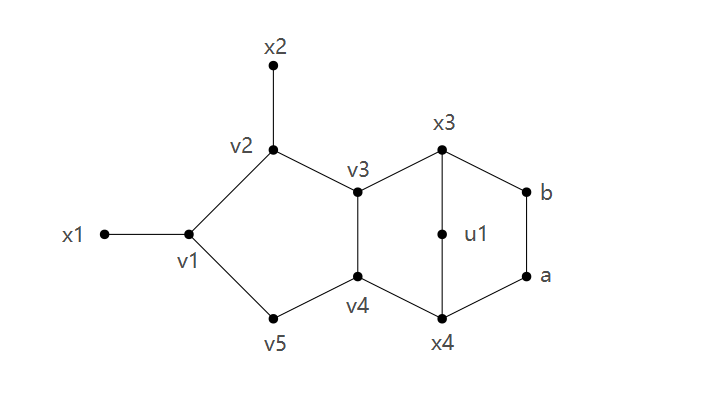
\includegraphics[width=0.6\textwidth]{figure/pcupqboundsaface.png} 
            \caption{Path is $x_4u_1u_2v_3$.} %最终文档中希望显示的图片标题
            \label{figure} %用于文内引用的标签
        \end{figure}
        Then $u_2 = x_3$. As discussed in \textbf{Lemma 4.5.}, at most one of $x_3, x_4$ can lie on $C_2$. Therefore, $x_4u_1u_2(x_3)v_3v_4$ would form a separating cycle of length five, which is a contradiction.
    \end{itemize}
    \end{proof}
    
    \item[Case 2:]\textit{\textbf{$P \cup Q$ is a separating cycle in $G$.}} It results that $P \cup Q$ is not a subgraph of $G_2$, for every cycle of length at most six in $G_2$ bounds a face.  
    
    \begin{claim}
    At most one of $\{x, y\}$ can lie on $C_2$.
    \end{claim}
\begin{proof}
    Let's recall the following two cases:
    \begin{itemize}
        \item[(1)] \textit{\textbf{$\{x, y\} = \{x_2, v_5\}$}}: As pointed out in the \textbf{Lemma 4.5.}, if $v_5 \in V(C_2)$, $x_2$ can not belong to $C_2$.
        \item[(2)] \textit{\textbf{$\{x, y\} = \{x_3, x_4\}$}}: As mentioned in the \textbf{Lemma 4.5.} that at least one of $x_3$ and $x_4$ is not on $C_2$.
    \end{itemize}
\end{proof}
Thus, we may assume that $x_4 \in C_2$ and $x_3 \notin C_2$. Meanwhile, a subpath $R$ of $P \cup Q$ of length exactly four joins $w_1, w_4 \in V(C_2)$. 
\begin{figure}[H] %H为当前位置,!htb为忽略美学标准,htbp为浮动图形
    \centering %图片居中
    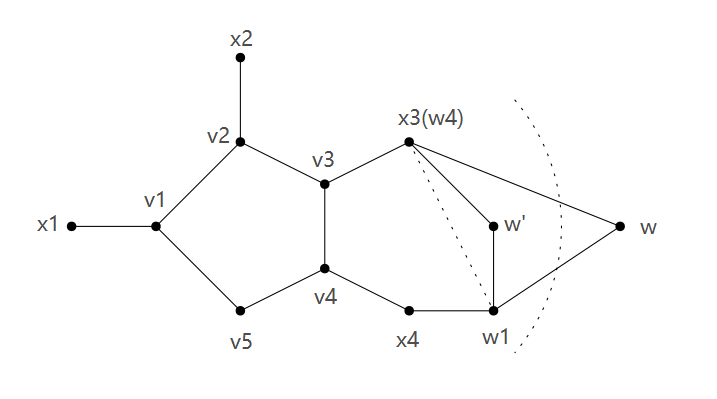
\includegraphics[width=0.7\textwidth]{figure/lemma2.2.png} 
    \caption{$P \cup Q$ is a separating cycle} %最终文档中希望显示的图片标题
    \label{figure} %用于文内引用的标签
    \end{figure}
Observed that the vertex $w \in (P \cup Q) \backslash V(G_2)$ is adjacent to $w_1$ and $w_4$. Let's take care of the position of $w$: assume firstly that $w \notin V(G_1)$, which implies that $w_1, w_4 \in V(C_1)$ because $w_1, w_4 \in V(C_2)$. Otherwise, edges $ww_1$ and $ww_4$ will build crosses with $C_1$. From the \textbf{Figure 20.} informed that $w_1$ and $w_4$ cannot be adjacent on the grounds that if this would not be the case, $w_1w_4w$ will form a triangle, which is a contradiction. Thereby, there is a common neighbor of $w_1$ and $w_4$ in $C_2$ which can replace $w$. So we suppose that $w \in V(G_1)$.

\begin{figure}[H] %H为当前位置,!htb为忽略美学标准,htbp为浮动图形
    \centering %图片居中
    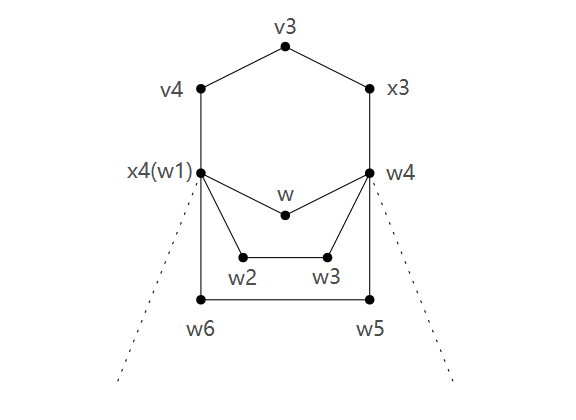
\includegraphics[width=0.6\textwidth]{figure/temp1.png} 
    \caption{$C_2$: $w_1w_2w_3w_4w_5w_6$ } %最终文档中希望显示的图片标题
    \label{figure} %用于文内引用的标签
\end{figure}
Provided that there is common neighbor $w_2$ of $w_1, w_4$, $R$ can be completed by $w_1w_2w_4$, which is a contradiction to the choice of $C_2$. Hence, we conclude that there are two vertices $w_2, w_3$ between $w_1$ and $w_4$ as in \textbf{Figure 21}. Let $w_1w_2w_3w_4w_5w_6$ be the vertices of $C_2$. What's more, we assume that $w_1w_2w_3w_4w$ forms a 5-face as well. In addition, $P \cup Q$ doesn't contains $w_5, w_6$ as shown in \textbf{Figure 21}. At the same time, $P \cup Q$ doesn't contain any vertex $v \in V(G) \backslash V(G_2)$ except $w$. $w_1, w_4$??
\end{itemize}
\end{proof}
%----------------------------------------------------------------------
\begin{theorem}[Grötzsch's theorem]
Every triangle-free planar graph is 3-colorable. \cite{grotzsch1959dreifarbensatz}
\end{theorem}
\begin{proof}
Let $G$ as stated to be a triangle-free graph and we'll prove this theorem by induction.\\
\textbf{Case 1: } If the minimum degree is smaller than three, which means it can be one or two.
\begin{itemize}
    \item if the minimum degree is one: search for vertices $\forall v \in V = \{v | deg(v) = 1\}$ and remove them from $G$ to get a new graph $G^{'}$. If the minimum degree of $G$ is two, then consider the case 1.2. Otherwise, we can apply the algorithm on $G^{'}$ and color $G^{'}$. Lastly, we can assign randomly a color different from the color of neighbor $\forall u \in \{u$ | $u$ is the neighbor of $v$, $\forall v \in V \}$ to $v$. 
    
    \item if the minimum degree is two: assume the vertex is $v \in V(G)$ and its neighbors $u, w \in V(G)$. Analogous to the former case, we remove the vertex $v$ from $G$ to obtain the new graph $G^{'}$. Suppose the coloring of $u, w$ is $c_1$ and $c_2$. If $c_1 = c_2$, then we can color $v$ randomly with a color different from $c_1(c_2)$. But if $c_1 \ne c_2$, we can accordingly assign $c_3$ to $v$. 
\end{itemize}
\textbf{Case 2:}  If every vertex $v$ has degree at least 3, we can apply lemma 4.3 on it. Thus, the theorem follows the induction on $G \backslash v$ by identifying pairs diagonally opposite vertices. And the way of coloring is already shown in the third section \textbf{Safety of multigram}: reconstruction step. 

\end{proof}
%----------------------------------------------------------------------
\section{Graph representation}
We'll use the same graph representation as in the third section from the original paper. \cite{dvorak2013threecoloring}

%----------------------------------------------------------------------
\section{The linear-time algorithm}
\subsection{Definitions}
As explained in the second section that in our algorithm, we will find some reducible multigrams to cut down the size of graph $G$. The difficulty now is how to efficiently check whether the found multigrams are safe, for which we will introduce another concept called \textit{security} that allows us testing safety in constant time. Before that, let's give a few more definitions:
\begin{definition}
A \textit{monogram} in the graph $G$ is the one-vertex sequence consisting of a vertex $v \in V(G)$ and has degree at most two. \cite{dvorak2013threecoloring} 
\end{definition}
Let $G$ be a triangle-free planar graph, $k \in \{1, 4, 5, 6\}$ and $\gamma = (v_1, ..., v_k)$ a mono-, tetra-, penta- or hexagram in $G$. Let $C$ be the subgraph of $G$.

\begin{definition}
A vertex $v \in V(G)$ is \textit{big}, if it has degree at least 60 and \textit{small} otherwise. \cite{dvorak2013threecoloring}
\end{definition}

\begin{definition}
A vertex $v \in V(G)$ is called \textit{$C$-admissible}, if $v$ is small and $v \notin C$; otherwise called \textit{$C$-forbidden}. \cite{dvorak2013threecoloring} 
\end{definition}

\begin{definition}
A pentagram $(v_1, v_2, v_3, v_4, v_5)$ is a \textit{decagram} if $v_5$ has degree exactly three as well. A tetragram $(v_1, v_2, v_3, v_4)$ is \textit{octagram} if all vertices have degree three. \cite{dvorak2013threecoloring}
\end{definition}
Furthermore, we extend the concept multigram as follows: a \textit{multigram} is a monogram, tetragram, pentagram, hexagram, octagram or decagram.

\begin{definition}
Let $\gamma$ be a multigram $(v_1, v_2, ..., v_k)$. The vertex $v_1$ is called \textit{pivot} of multigram. \cite{dvorak2013threecoloring}
\end{definition}
\subsection{Security of multigrams}
Next, we'll explain what's the meaning of $C$-secure and define a smaller graph $G^{'}$ which is called \textit{$\gamma$-reduction of $G$}.

\begin{itemize}
    \item[(1)] \textit{\textbf{$\gamma$ is a monogram}}. We define it to be always safe. $\gamma$ is $C$-secure, if $v_1 \notin V(C)$ and $G^{'} := G \backslash v_1$.
    \item[(2)] \textit{\textbf{$\gamma$ is a tetragram}}. 
    \begin{figure}[H] %H为当前位置,!htb为忽略美学标准,htbp为浮动图形
    \centering %图片居中
    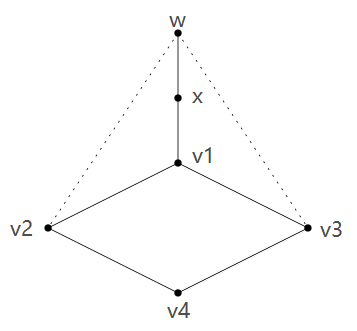
\includegraphics[width=0.4\textwidth]{figure/Csecuretetagram.png} 
    \caption{$C$-secure tetragram} %最终文档中希望显示的图片标题
    \label{figure} %用于文内引用的标签
    \end{figure}
    $\gamma$ is $C$-secure if 
        \begin{itemize}
            \item $\gamma$ is safe,
            \item $v_1$ is $C$-admissible and has degree exactly three,
            \item letting $x$ be the neighbor of $v_1$ other than $v_2$ and $v_4$, the vertex $x$ is $C$-admissible,
            \item either
                \begin{itemize}
                    \item $v_3$ is $C$-admissible, or
                    \item every neighbor $w$ of $x$ is $C$-admissible or belongs to a 4-face incident with the edge $v_1x$ (either $v_1v_2wx$ or $v_1v_4wx$).
                \end{itemize}
        \end{itemize}
        $G^{'}$ be the graph obtained by identifying vertices $v_1$ and $v_3$ and delete one edge from each f the two pairs of parallel edges. 
    \item[(3)] \textit{\textbf{$\gamma$ is an octagram}}. We define it to be always safe as well. $\gamma$ is $C$-secure, if $v_1, v_2, v_3, v_4$ are $C$-admissible. $G^{'} := G \backslash \{v_1, v_2, v_3, v_4\}$.
    \item[(4)] \textit{\textbf{$\gamma$ is a decagram}}. $\forall i \in \{1, 2, 3, 4\}$, $x_i$ is the neighbor of $v_i$ other than $v_{i-1}$ and $v_{i+1}$, where $v_0 = v_5$. The decagram $\gamma$ is \textit{safe}, if 
    \begin{itemize}
        \item $x_1, x_3$ are distinct and non-adjacent,
        \item there is no path of length two between them.
    \end{itemize}
    The decagram $\gamma$ is $C-$secure, if 
    \begin{itemize}
        \item $\gamma$ is safe,
        \item $v_1, v_2, v_3, v_4, v_5, x_1, x_3$ are $C$-admissible.
    \end{itemize}
    $G^{'}$ is obtained from $G \backslash \{v_1, v_2, v_3, v_4, v_5\}$ by adding the edge $x_1x_3$.
    
    \item[(5)] \textit{\textbf{$\gamma$ is a pentagram}}. $\forall i \in \{1, 2, 3, 4\}$, $x_i$ is the neighbor of $v_i$ other than $v_{i-1}$ and $v_{i+1}$, where $v_0 = v_5$.
    $\gamma$ is $C$-secure, if 
        \begin{itemize}
            \item $v_1, v_2, v_3, v_4, v_5, x_1, x_2, x_3, x_4$ are $C$-admissible,
            \item either $v_5$ or $x_2$ has no $C$-forbidden neighbor,
            \item either $x_3$ or $x_4$ has no $C$-forbidden neighbor.
        \end{itemize}
    $G^{'}$ is obtained from $G \backslash \{v_1, v_2, v_3, v_4\}$ by identifying $v_5$ and $x_2$; $x_3$ and $x_4$. If $x_3$ and $x_4$ should have a common neighbor, then delete one of the parallel edges.  
    
    \item[(6)] \textit{\textbf{$\gamma$ is a hexagram}}. $\gamma$ is $C$-secure, if
    \begin{itemize}
        \item $v_1, v_3, v_6$ are $C$-admissible,
        \item $v_1$ has degree exactly three,
        \item the neighbor of $v_1$ other than $v_2$ or $v_6$ is $C$-admissible.
    \end{itemize}
    $G^{'}$ be the graph obtained by identifying vertices $v_1$ and $v_3$ and delete one edge from each f the two pairs of parallel edges. 
\end{itemize}

\begin{definition}
A \textit{null graph} is a graph which consists only the isolated vertices. \cite{null}
\end{definition}

\begin{definition}
A multigram is \textit{secure}, if it is $K_0$-secure, where $K_0$ is the null graph. \cite{dvorak2013threecoloring}
\end{definition}

\subsection{Constant-time operations}
Noted that the followings lemmas will not be proved in this paper, see proofs from the original paper.\cite{dvorak2013threecoloring}
\begin{lemma}
Let $G$ be a triangle-free plane graph, let $\gamma$ be a safe multigram in $G$, and let $G^{'}$ be the $\gamma$-reduction of $G$. Then $G^{'}$ is triangle-free, and every 3-coloring of $G^{'}$ can be converted to a 3-coloring of $G$ in constant time. Moreover, if $\gamma$ is secure, then $G^{'}$ can be regarded as having been obtained from $G$ by deleting at most 126 edges, adding at most 116 edges, and deleting at least one isolated vertex.\cite{dvorak2013threecoloring}
\end{lemma}

\begin{definition}
\textit{Two small vertices $u, v \in V(G)$ are close} if either there is a path of length at most four between $u$ and $v$ consisting of small vertices, or a facial cycle of length at most six contains both $u$ and $v$. \textit{A vertex $u$ is close to an edge $e$} if both $u$ and $e$ belong to the facial walk of the same face and the distance between $u$ and and one end of $e$ in this facial walk is at most two. \cite{dvorak2013threecoloring}
\end{definition}

\begin{claim}
Every vertex $v$ there are at most $1 + 4 \cdot 59 + 59^{2} + 59^{3} + 59^{4}$ vertices that are close to $v$, and for every edge $e$, there are at most 10 vertices that are close to $e$. \cite{dvorak2013threecoloring}
\end{claim}
\begin{proof}
    
    \begin{figure}[htbp]
    \centering
    \begin{minipage}[t]{0.48\textwidth}
    \centering
    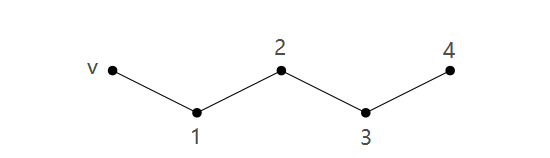
\includegraphics[width=1\textwidth]{figure/592.png}
    \caption{Case 1}
    \end{minipage}
    \begin{minipage}[t]{0.28\textwidth}
    \centering
    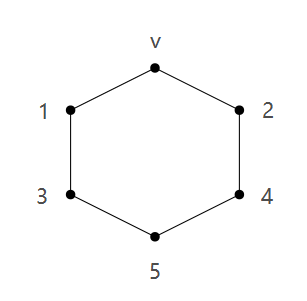
\includegraphics[width=1\textwidth]{figure/591.png}
    \caption{Case 2}
    \end{minipage}
    \end{figure}
    Observed that in the \textbf{Figure 23}, vertex 1 can have at most 59 neighbors, vertex 2 can have at most $59^{2}$ neighbors, vertex 3 can have at most $59^{3}$ neighbors and vertex 4 can have at most $59^{4}$ neighbors. In the \textbf{Figure 24}, vertex 1 and 2 can totally have at most 59 neighbors, while vertex 3 and 4 each can have 59 neighbors. But vertex 5 can have only one vertex. So all things considered there are at most $1 + 4 \cdot 59 + 59^{2} + 59^{3} + 59^{4}$ vertices that are close to $v$.
    \begin{figure}[H] %H为当前位置,!htb为忽略美学标准,htbp为浮动图形
    \centering %图片居中
    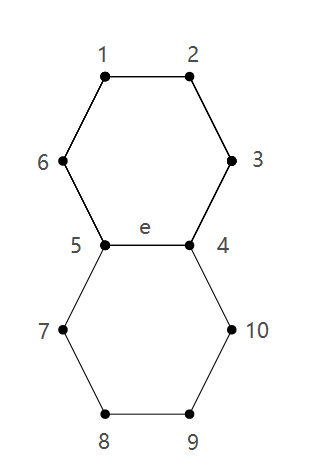
\includegraphics[width=0.28\textwidth]{figure/593.png} 
    \caption{Vertices close to edge $e$} %最终文档中希望显示的图片标题
    \label{figure} %用于文内引用的标签
    \end{figure}
    Noted that both $v$ and $e$ have to belong to the same walk of the same face. In addition, there are at most two faces that incident with edge $e$, which follows that there are at most 10 vertices that are close to edge $e$.
\end{proof}

\begin{lemma}
Given a triangle-free plane graph $G$ and a vertex $v \in V(G)$, it can be decided in constant time whether $G$ has a secure multigram with pivot $v$. \cite{dvorak2013threecoloring}
\end{lemma}

\begin{lemma}
Let $G$ and $G^{'}$ be triangle-free plane graphs, such that for some pair of non-adjacent vertices $u, v \in V(G)$ the graph $G^{'}$is obtained from $G$ by adding the edge $uv$. Let $\gamma$ be a secure multigram in exactly one of the graphs $G$, $G^{'}$. Then the pivot of $\gamma$ is close to $u$ or $v$ in $G$, or to the edge $uv$ in $G^{'}$. \cite{dvorak2013threecoloring}
\end{lemma}

\begin{theorem}
Every non-null triangle-free planar graph has a secure multigram.
\end{theorem}
\begin{proof}
See the proof from the original paper. \cite{dvorak2013threecoloring}
\end{proof}

\subsection{The algorithm}
Now, let's focus on the linear-time algorithm with running time $\mathcal{O}(|V(G)|)$:
we may assume that the input graph is triangle-free, because we can use the algorithm which was designed by Hopcroft, John; Tarjan, Robert E \cite{10.1145/321850.321852} to test planarity in $\mathcal{O}(n)$ time by \textit{path addition method}. So it holds our algorithm's running time in linear-time. 
%%% Coloring the comment as blue
\newcommand\mycommfont[1]{\footnotesize\ttfamily\textcolor{blue}{#1}}
\SetCommentSty{mycommfont}

\SetKwInput{KwInput}{Input}                % Set the Input
\SetKwInput{KwOutput}{Output}              % set the Output

\begin{algorithm}[H]
\DontPrintSemicolon
  \KwInput{A triangle-free planar graph}
  \KwOutput{A 3-coloring of $G$}
  $L := \{v \in V(G) | deg(v) \leq 3\}$  \tcp*{L is a list}
  temp := $G$   \tcp*{Store the original graph $G$}
  \For{$v \in L$}    
    { 
         Remove $v$ from $L$ \\
    	\If{$G$ has a multigram with pivot $v$}
        {
            \Statex $\gamma$ := such safe multigram \\
            $G^{'}$ := $\gamma$-reduction of $G$ \\
            \For{every edge $uv$ deleted or added during construction of $G^{'}$}{
                Add to $L$ all vertices that are close to $u$ or $v$ or to the edge $uv$ in $G$ or $G^{'}$
            }
            $G$ := $G^{'}$ \tcp*{To reduce the size of $G$}
        }
        \Else{
            continue to next iteration
        }
    }
   \While{G $\ne$ temp} 
   {
        Color the graph $G$ \tcp*{Reconstruction step}\\
   		Convert the 3-coloring of $G$ to the graph $G^{'}$ before the $\gamma$-reduction \\
   		$G$ := $G^{'}$
   }
\caption{3-coloring in triangle-free planar graph}
\end{algorithm}
\begin{proof}[Description] We initialize $L$ as the list of vertices with degree at most three. During the execution of the algorithm, $L$ includes all pivots of all secure multigrams. The algorithm works as follows: remove randomly a vertex $v$ from $L$ and check whether there is a multigram whose pivot is $v$, which can be done in constant time according to \textbf{Lemma 6.2.} If there is no such multigram, then we go to the next iteration. Otherwise, let $\gamma$ be such multigram and $G^{'}$ be the $\gamma$-reduction of $G$, which can be done in constant time according to \textbf{Lemma 6.1.} \textbf{Lemma 6.3.} can guarantee that $L$ includes all pivots of all secure multigrams. After we get the coloring of $G^{'}$, it can be converted to the coloring of $G$. And we'll do this until we get the coloring of the original input graph $G$. Noticed that the number of vertices added to $L$ is proportional to the number of vertices removed from $G$. Hence, the running time is $\mathcal{O}(|V(G)|)$, as desired.
\end{proof}

\begin{algorithm}[H]
\DontPrintSemicolon
  \KwInput{A triangle-free plane graph $G$, a facial cycle $C$ in $G$ of length at most
five, and a proper 3-coloring $\phi$ of $C$.}
  \KwOutput{A proper 3-coloring of $G$ whose restriction to $V(C)$ is equal to $\phi$.}
\caption{3-coloring in triangle-free planar graph with coloring constraint}
\end{algorithm}
\begin{proof}[Description] 
The description is exactly the same, except that we replace
“secure” by “$C$-secure” and appeal to \textbf{Lemma 7.1} rather than \textbf{Theorem 6.4.} And its running time is still $\mathcal{O}(|V(G)|)$.\cite{dvorak2013threecoloring}
\end{proof}

\subsection{Implementation}
%----------------------------------------------------------------------
\section{Proof of correctness}
\begin{definition}
\textit{$f$ is opposite to $xy$}, if $xy$ is an edge in a planar graph, and $f$ is a face of $G$ incident with $y$ but not with the edge $xy$. Noted that this definition is not symmetric: $f$ is opposite to $xy$, but $f$ is \textit{not} opposite to $yx$. \cite{dvorak2013threecoloring}
\begin{figure}[H] %H为当前位置,!htb为忽略美学标准,htbp为浮动图形
\centering %图片居中
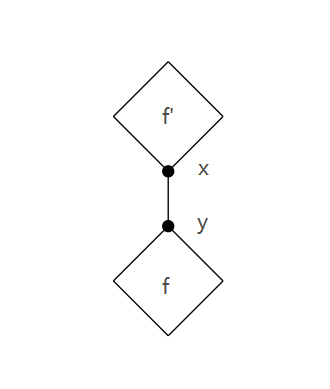
\includegraphics[width=0.3\textwidth]{figure/opposite.png} 
\caption{$xy$-opposite and $yx$-opposite faces} %最终文档中希望显示的图片标题
\label{figure} %用于文内引用的标签
\end{figure}
\end{definition}

\begin{lemma}
Let $G$ be a connected triangle-free planar graph and let $f_0$ be its
outer face. Assume that $f_0$ is bounded by a cycle $C$ of length at most six,
$V(G) \ne V (C)$, and if $C$ has length six, then $|V(G) - V(C)| \geq 2$. Then $G$
contains a $C$-secure multigram. \cite{dvorak2013threecoloring}
\end{lemma}

\begin{proof}
By contradiction, presuming that $G$ is a counterexample with $E(G)$ minimum, namely $G$ doesn't contain any $C$-secure multigram.

\begin{corollary}
If $K \ne C$ is a cycle in $G$ of length at most six, then $K$ bounds a face,
or $K$ has length six and the open disk bounded by $K$ contains at most
one vertex. \cite{dvorak2013threecoloring}
\end{corollary}
We conclude that $C$ is induced and every tetragram is safe the reason is that from \textbf{Corollary 7.1.1.}, we know that a cycle in $G$ of length four will bound a face. Hence, according to \textbf{Claim 4}, those tetragram is always safe.\\ 

Next, we assign the following charges to the vertices and faces of $G$. Primitively, a vertex $v \in V(G)$ will obtain a charge of 
\begin{equation*}
\left\{
    \begin{array}{ll}
    9 \ deg(v) -36, & v \notin V(C)  \\
    8 \ deg(v) - 19, & otherwise
    \end{array}
\right.
\end{equation*}
and a face will take a charge of 
\begin{equation*}
\left\{
    \begin{array}{ll}
    0, &  f = f_0\\
    9\ell -36, & f \neq f_0 \ and \ f \ has \ length \ \ell
    \end{array}
\right.
\end{equation*}

\begin{claim}
The sum of charges is negative.
\end{claim}
\begin{proof}
\begin{align*}
    & sum \ of \ charges \ = \sum_{v \notin V(C)}9\big(deg(v) - 4\big) + \sum_{v \in V(C)} \big(8 \ deg(v) - 19\big) + \sum_{f \neq f_0}9\big(size(f) - 4\big) \\
    &= \underbrace{\sum_{v \in V(G)}9\big(deg(v) - 4\big) - \sum_{v \in V(C)}9\big(deg(v) - 4\big)}_{\sum_{v \notin V(C)}9\big(deg(v) - 4\big)} + \sum_{v \in V(C)} \big(8 \ deg(v) - 19\big) + \sum_{f \neq f_0}9\big(size(f) - 4\big) \\
    &= \sum_{v \in V(G)}9\big(deg(v) - 4\big) + \sum_{f \neq f_0}9\big(size(f) - 4\big) - \sum_{v \in V(C)}(deg(v) - 17)\\
    &= \sum_{v \in V(G)}9\big(deg(v) - 4\big) + \sum_{f \neq f_0}9\big(size(f) - 4\big) - \sum_{v \in V(C)}deg(v) + 17\left| V \right|\\
    &= \sum_{v \in V(G)}9\big(deg(v) - 4\big) + \sum_{f}9\big(size(f) - 4\big) - 9(size(f) - 4) - \sum_{v \in V(C)}deg(v) + 17\left| V(C) \right|\\
    &= \sum_{v \in V(G)}9\big(deg(v) - 4\big) + \sum_{f}9\big(size(f) - 4\big) - 9 \left| V(C) \right| + 36 - \sum_{v \in V(C)}deg(v) + 17\left| V(C) \right|\\
    &= \underbrace{18 \left| E \right| - 36\left| V(G) \right| + 18 \left| E \right| - 36 \left| F \right|}_{\text{apply Euler's formula here: v + f - e = -2}} - \sum_{v \in V(C)}deg(v) + 8 \left| V(C) \right| + 36 \\
    &= -36 \cdot 2 - \sum_{v \in V(C)}deg(v) + 8 \left| V(C) \right| + 36\\
    &= 8 \left| V(C) \right| - 36 - \sum_{v \in V(C)}deg(v)\\
    &\leq 8 \left| V(C) \right|- 2 \left| V(C) \right| - 1 - 36 \\
    &\leq -1 \ (since \ the \ length \ of \ C \ is \ at \ most \ 6)
\end{align*}

The reason of first inequality is that all vertices of cycle $C$ have at least degree two and there is at least one vertex of $C$ whose degree is at least three, which follows $\sum_{v \in V(C)}deg(v) \leq 2\left| V(C) \right| + 1$. \\
\end{proof}

\begin{definition}
Two edges $e_1$, $e_2$ in $G$ are \textit{consecutive}, if they form a path in $G$. \cite{BUJTAS2012561}
\end{definition}

\begin{definition}
Assume $f$ $\neq$ $f_0$ is a face contained in $G$ incident with a vertex $v \in V(C)$. Provided that there exist two consecutive edges within the boundary of $f$ such both are incident with $v$ and neither belongs to $C$, then we are saying that $f$ is a $v-interior \
face$. \cite{dvorak2013threecoloring}
\end{definition}

\begin{figure}[H] %H为当前位置,!htb为忽略美学标准,htbp为浮动图形
\centering %图片居中
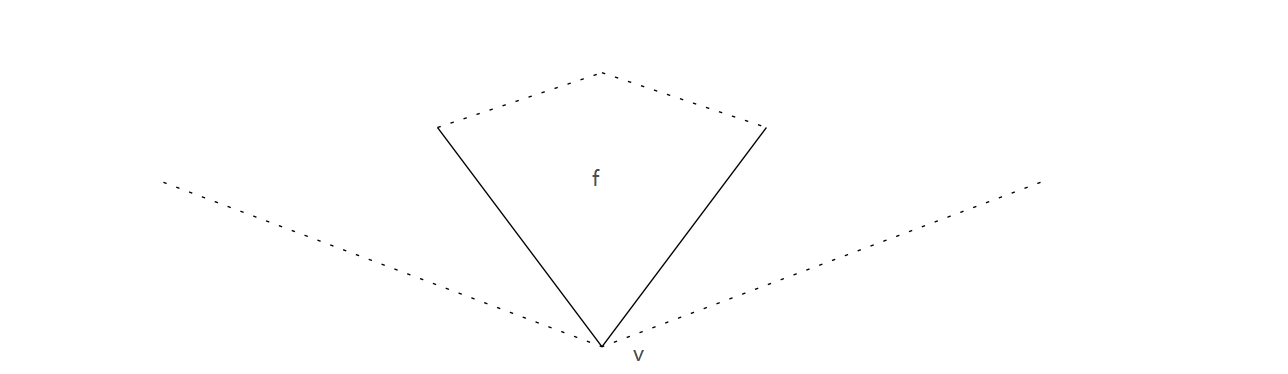
\includegraphics[width=1\textwidth]{f-interior.png} 
\caption{$v$-interior face $f$} %最终文档中希望显示的图片标题
\label{figure} %用于文内引用的标签
\end{figure}

\begin{corollary}
If at least $k$ vertices of $C$ have degree at least three, then the sum of the
charges is at most -$k$. \cite{dvorak2013threecoloring}
\end{corollary}

We now redistribute the charges consistent with the subsequent rules.
The rules are:\cite{dvorak2013threecoloring}
\begin{itemize}
    \item[\textbf{(A)}] Every face other than $f_0$ sends three units of charge to every incident vertex $v$ such that either $v$ $\in$ $V(C)$ and $v$ has degree two in $G$, or $v$ $\notin$ $V(C)$ and $v$ has degree exactly three.
    \item[\textbf{(B)}] Every big vertex not on $C$ sends three units to each incident face, and
four units to each 4-face that shares an edge with $C$.
\item[\textbf{(C)}] Every vertex $v \in V(C)$ sends three units to every $v$-interior face.
\item[\textbf{(D)}] If $x \in V(G)$ is $C$-forbidden, and $y$ is a $C$-admissible neighbor of $x$ of
degree three, then $x$ sends three units to the unique face opposite to $xy$,
and one unit to the face opposite to $yz$ for every $C$-admissible neighbor
$z$ of $y$ of degree three.
\item[\textbf{(E)}] Every $C$-forbidden vertex sends five units to every $C$-admissible neighbor
of degree at least four.
\item[\textbf{(F)}] For every $C$-admissible vertex $y$ of degree at least four that has a $C$-forbidden neighbor we select a $C$-forbidden neighbor $x$ of $y$ and let $y$
send one unit to each face opposite to $xy$, and one unit to the face
opposite to $yz$ for every $C$-admissible neighbor $z$ of $y$ of degree three.
\end{itemize}
Since $G$ is a counterexample of the lemma, $G$ doesn't contain any $C$-secure multigram, which follows that every vertex $v \in V(G)$ has degree at least two and the vertices with degree two are on $C$. 
\begin{claim}
Every vertex $v \in V(G)$ with degree $d$ has non-negative charge.
\end{claim}

\begin{proof}
We will observe the following cases:
\begin{itemize}
    \item[Case 1.1:] \textit{\textbf{$v$ is $C$-admissible and $d = 3$.}} At the beginning, $v$ has the charge $9 \cdot 3 - 36 = -9$. Pursuant to the rule (A), $v$ will get totally 9 units from three incident faces other than $f_0$, which results that the final charge of $v$ is zero (non-negative).
    \item[Case 1.2.1:] \textit{\textbf{$v$ is $C$-admissible, $d \geq 4$ and has no $C$-forbidden neighbor.}} The original charge of $v$ is $9d - 36 \geq 0$. What's more, $v$ doesn't send out any charges. So the final charge is still non-negative.
    \item[Case 1.2.2:] \textit{\textbf{$v$ is $C$-admissible, $d \geq 4$ and has a $C$-forbidden neighbor.}} Let $x$ be the $C$-forbidden neighbor of $v$. Informed from the rule (E) that $v$ will receive five units from $x$. Meanwhile, $v$ sends out at most (2$d$ - 3) units according to the rule (F).
    
    \begin{figure}[H] %H为当前位置,!htb为忽略美学标准,htbp为浮动图形
        \centering %图片居中
        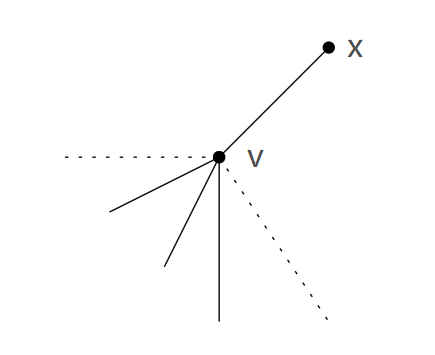
\includegraphics[width=0.3\textwidth]{figure/lemma_5.1.2_2d-3.png} 
        \caption{Case 1.2.2} %最终文档中希望显示的图片标题
        \label{figure} %用于文内引用的标签
    \end{figure}
    Noticed that $v$ has remaining ($d - 1$) neighbors except $x$. In the worst case, all ($d - 1$) neighbors have degree exactly three. Thus, $v$ will send out at most ($d - 1$) units to each face $f$ that $f$ is opposite to $vz$, $\forall z \in Z$, where $Z$ is the set of all neighbors of $v$ except x. Furthermore, observed from \textbf{Figure 28} that, ($d - 1$) edges(neighbors) can at most form ($d - 2$) $xv$-opposite faces. As a result, $v$ sends out at most ($d - 2 + d - 1$) = $2d - 3$ units.\\
    $\longrightarrow$ The final charge of $v = 9d - 36 + 5 - (2d - 3) = 7d - 28 \geq 0$ is also non-negative.
    \item[Case 2.1:] \textit{\textbf{$v$ is big and $v \notin C.$}} As stated in the rule (B), $v$ sends $3d$ units to all incident faces and at most 4$\cdot$6 = 24 units to all 4-faces that share an edge of $C$, since $C$ has length at most six. Additionally, $v$ sends at most 5$d$ units using the rule (D),
    \begin{figure}[H] %H为当前位置,!htb为忽略美学标准,htbp为浮动图形
        \centering %图片居中
        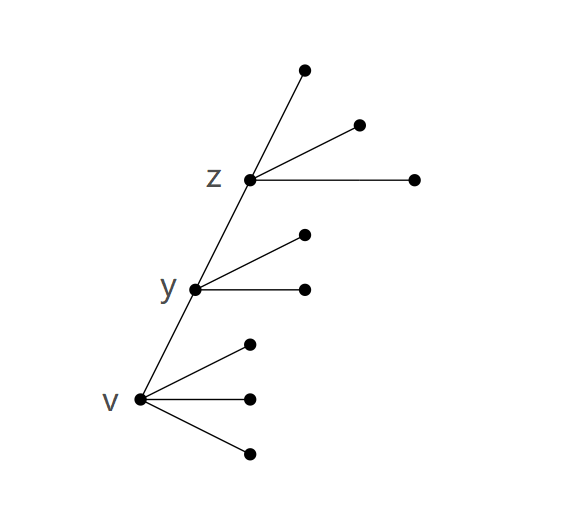
\includegraphics[width=0.4 \textwidth]{figure/lemma_5.1.2_5d.png} 
        \caption{Case 2.1 using the rule (D)} %最终文档中希望显示的图片标题
        \label{figure} %用于文内引用的标签
    \end{figure}
    The reason is that each neighbor $y$ of $v$ can have degree three and be $C$-admissible which can form at most two unique faces opposite to $vy$. In addition, every vertex $y$ can have at most three neighbors. Each neighbor $z$ can also be $C$-admissible of degree three. Hence, there are at most three faces opposite to $yz$ for each $y$. In conclusion, $v$ sends out at most five units for each neighbor, which deduces $v$ can send at most 5$d$ units using rule (D). Or using rule (E), provided that all neighbors of $v$ can be $C$-admissible and have degree at least 4. As a consequence, the final charge of $v$ = $9d -36 - 3d - 24 - 5d = d - 60 \geq 0$, since $v$ is big.
    \item[Case 2.2:] \textit{\textbf{$v \in C.$}} The charge of $v$ at the beginning is $8d - 19$. Noted that if $d = 2$, by the rule (A), $v$ will receive three units. So we assume that is not the case. Otherwise, according to rule (A), $v$ sends out 3($d-3$) units by the rule (C), because $v$ has two neighbors that are on $C$, which leads that the remaining ($d-2$) neighbors can form ($d - 3$) $v$-interior faces. Besides, $v$ sends 5($d - 2$) units using rule (D) or (E). The argument is similar to the former case 2.2: there are at most ($d-2$) $C$-admissible neighbors of $v$. In consequence, the final charge of $v$ = $8d - 19 - 3(d - 3) - 5(d - 2) = 0$.
\end{itemize}
\end{proof}

\begin{claim}
Every face of length $\ell \geq 6$ has non-negative final charge.
\end{claim}
\begin{proof}
Noticed from rule (A) that each face $f \ne f_0$ can just send at most 3$\ell$ units. So the final charge = $9\ell - 36 - 3\ell = 6\ell - 36 \geq 0$. 
\end{proof}
From the \textbf{Claim 9} we prove that there is a face $f \ne f_0$ in G of length at most five that has strictly negative final charge.

\begin{corollary}
No vertex incident with $f$ has degree two. \cite{dvorak2013threecoloring}
\end{corollary}

\begin{proof}
Prove using contradiction: there is a vertex $v$ incident with $f$ with degree exactly two. Thereby, $v$ and the two incident edges are on $C$, which implies that there are at least two vertices of $f$ are on $C$ that will not receive any charges from $f$. Because of the fact that the face $f$ has strictly negative final charge, we deduce that the length of $f$ is four:
\begin{align*}
    The \ final \ charge &= 9\ell -36 - \big(1 \cdot 3 + (\ell - 2 - 1) \cdot 3\big) < 0\\
    &\Longrightarrow \ell < 5\\
    &\Longleftrightarrow \ell \leq 4 
\end{align*}
Let $u_1u_2u_3u_4$ be the bounded face, where $u_1u_2u_3$ are consecutive vertices of $C$ and $u_2$ has degree exactly two. Meanwhile, $u_4 \notin C$, since $C$ is induced. Then $u_4$ is small and hence $C$-admissible. The reason is that if $u_4$ would be big, by using rule (B), $u_4$ would send seven units to $f$. Furthermore, $f$ has initial charge $9\cdot4 - 36 = 0$ and $f$ sends three units to $u_2$ by rule (A). As a result, the final charge of $f$ would be $0 - 3 + 7 = 4$, which is a contradiction. Let $C^{'}$ be the cycle obtained from $C$ by replacing the vertex $u_2$ by $u_4$. Since we replace $u_2$ by $u_4$, it follows $|V(C^{'})| = |V(C)| \leq 6$. So the length constraint holds.
\begin{figure}[H] %H为当前位置,!htb为忽略美学标准,htbp为浮动图形
    \centering %图片居中
    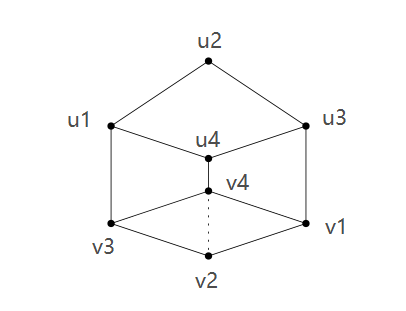
\includegraphics[width=0.4 \textwidth]{figure/corollary3.png} 
    \caption{Cycle $C$ and $C^{'}$} %最终文档中希望显示的图片标题
    \label{figure} %用于文内引用的标签
\end{figure}
As above mentioned, $u_4$ has degree at least three, $C^{'}$ can't form a face, which follows from \textbf{Corollary 7.1.1} that $C^{'}$ has length six and contains exactly one vertex $v_4$. Next, we order the remaining three vertices on $C$ as in \textbf{Figure 30} with $v_1v_2v_3$ so that the original cycle $C$ is $u_1u_2u_3v_1v_2v_3$ and $v_4$ is adjacent to $u_4, v_1, v_3$. Observed that:
\begin{itemize}
    \item[(1)] ($u_4, u_1, u_2, u_3$) is safe, since there is not path at most three other than $u_4u_1u_2$ and $u_4u_3u_2$ that ends with $u_2$ and $u_4$. 
    \item[(2)] As proved above, $u_4$ is $C$-admissible and has degree exactly three.
    \item[(3)] Noticed from the figure that the neighbor $v_4$ of $u_4$ is not on $C$ and has degree exactly three as well. It follows that $v_4$ is also $C$-admissible.
    \item[(4)] $v_4$ belongs to the 4-face($u_4, u_1, v_3, v_2$) incident with $u_4v_4$. 
\end{itemize}
Resultantly, ($u_4, u_1, u_2, u_3$) is a $C$-secure tetragram, which is a contradiction to the supposition that there is no $C$-secure multigram in $G$.
\end{proof}

\begin{definition}
Let $uv$ be the edge to which $f$ is opposite. $v$ is a \textit{sink}, if $v$ has degree three and both $u$ and $v$ are $C$-admissible. $v$ is a \textit{source}, if either $v \notin V(C)$ and $v$ is big, or $v \in V(C)$ and $f$ is $v$-interior. \cite{dvorak2013threecoloring}
\end{definition}

\begin{observation}
$v$ is \textbf{not} a source, then either $v$ is small and $v \notin V(C)$; or $v \in V(C)$ and $f$ is not $v$-interior.
\end{observation}

\begin{observation}
The equivalences of definition of sink and source are stated as follows: \cite{dvorak2013threecoloring}
\begin{itemize}
    \item $v$ is a sink $\Longleftrightarrow$ $v$ has degree three and receives three units of charge from $f$ by rule (A) and $f$ does not receive three units by rule (D) from $u$.
    \item $v$ is a source $\Longleftrightarrow$ $v$ sends three units of charge to $f$ by rule (B) or (C).
\end{itemize}
\end{observation}
Suppose $s$ is the number of sources and $t$ is the number of sinks. Then we have the initial charge of $f$ $9 + 3s - 3t$, if the length of $f$ is five; $3s - 3t$, if the length of $f$ is four. 

\begin{itemize}
    \item[Case 1.1: ] \textit{\textbf{$f$ has length five and $v_5$ is $C$-admissible of degree three.}} Let $v_1v_2v_3v_4v_5$ be the cycle that bounds $f$. For $f$ has strictly negative final charge in the end, there are at least four sinks. Hence, we may assume that $v_1, v_2, v_3, v_4$ are sinks. In other word, they are $C$-admissible and have degree exactly three. In addition, ($v_1, v_2, v_3, v_4, v_5$) is a pentagram according to the definition. Let $x_i$ be the neighbor of $v_i$ except $v_{i-1}$ and $v_{i+1}$, $\forall i \in \{1, 2, 3, 4\}$, where $v_0 = v_5$. It infers that $x_1, x_2, x_3, x_4$ are distinct and pairwise non-adjacent. The reason is as follows:\\
    \textit{\textbf{(Case 1)}} If $x_i$ and $x_{i+1}$ would be adjacent, it will create a $C$-secure tetragram with vertices $v_i$ and $v_{i+1}$, which is a contradiction.\\
    \textit{\textbf{(Case 2)}} If $x_i$ and $x_{i+2}$ would be adjacent, from \textbf{Corollary 7.1.1.} that $x_ix_{i+2}v_{i+2}v_{i+1}v_{i}$ bounds a face. However, it contains a vertex $x_{i+1}$, which is a contradiction as well.\\
    Noticed from (Case 2) that there is no path from $x_1$ to $x_3$ with length two, then ($v_1, v_2, v_3, v_4, v_5$) is a $C$-secure decagram.
    
    
    
    \item[Case 1.2: ] \textit{\textbf{$f$ has length five and $v_5$ is not $C$-admissible of degree three.}} If there is a path from $x_1$ to $x_3$ of length three, then consider the cycle $K$ = $x_1v_1v_2v_3x_3y$. 
    \begin{figure}[H] %H为当前位置,!htb为忽略美学标准,htbp为浮动图形
        \centering %图片居中
        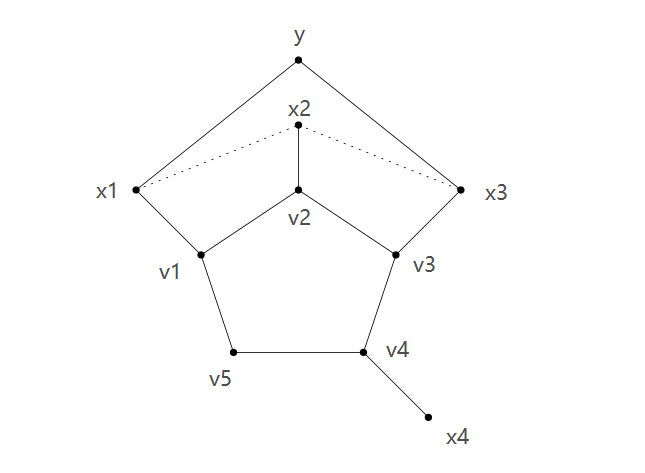
\includegraphics[width=0.6 \textwidth]{figure/contradictionpentagram.png} 
        \caption{Case 1.2} %最终文档中希望显示的图片标题
        \label{figure} %用于文内引用的标签
    \end{figure}
    Since the cycle $K$ has length six and from \textbf{Corollary 7.1.1.} that $K$ contains at most one vertex, it results that $v_4$ and $v_5$ are not inside $K$. Hence, either $y = x_2$ or $x_2$ is the vertex containing in the cycle $K$. Therefore, $x_2$ is adjacent to $x_1$ and $x_3$. In the former case, it's obvious true. In the latter case, we can prove it by contradiction: if $x_2$ is not adjacent to one of $x_1$ and $x_3$, it will form a triangle, which is against to the definition of planar graph. So in any case, $x_2$ is adjacent to $x_1$ and $x_3$, which is a contradiction to what we've proved in the case 1.1 that $x_1, x_2, x_3$ should be pairwise non-adjacent. 
\end{itemize}
Consequently, from both cases above that $v_5$ is either not $C$-admissible or has degree at least four, which implies that $v_5$ is not a sink and then the final charge of $f$ is at least $9 - 3 \cdot 4 = -3$. What's more. $v_5$ is not a source neither. If $v_5$ would be a source, then the final charge of $f$ would be zero, which is a contradiction to the negative final charge of $f$. Thus, it deduces from \textbf{Observation 5.} that $v_5$ is $C$-admissible and hence has degree at least four. We may claim that the pentagram $(v_1, v_2, v_3, v_4, v_5)$ is safe: 
\begin{itemize}
    \item there is a path of length at most three in $G \backslash \{v_1, v_2, v_3, v_4\}$ that ends with $x_2$ and $v5$, which can be completed via a path $v_5v_1v_2$ to be a new cycle $K$.
    \begin{figure}[H] %H为当前位置,!htb为忽略美学标准,htbp为浮动图形
        \centering %图片居中
        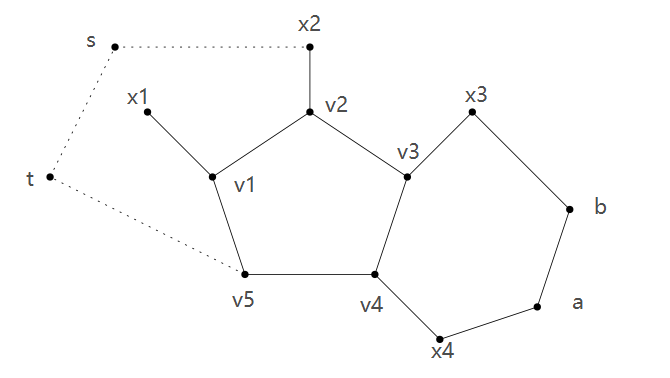
\includegraphics[width=0.6 \textwidth]{figure/case1.3.png} 
        \caption{Safe pentagram} %最终文档中希望显示的图片标题
        \label{figure} %用于文内引用的标签
    \end{figure}
From \textbf{Corollary 7.1.1.} that $K$ contains at most one vertex. On the grounds of this, $x_1$ is adjacent to $x_2$(the argument is the same as in the case 1.2), which is a contradiction.

\item considering the path of length at most three from $x_3$ to $x_4$ that can be completed to a cycle $K^{'}$ ($x_3v_3v_4x_4ab$) by the path $x_4v_4v_3x_3$ supposing that the length of cycle is six. Observed that $v_3, v_4$ are sinks, so $v_3$ has degree exactly three and $x_3, x_4$ are $C$-admissible. Thus, the hexagram ($v_4, v_3, x_3, b, a, x_4$) is $C$-secure, which is a contradiction. It follows that the path from $x_3$ to $x_4$ can only be two.
\end{itemize}
According to the above proof, we have shown that the pentagram $(v_1, v_2, v_3, v_4, v_5)$ is safe. By symmetry the pentagram $(v_4, v_3, v_2, v_1, v_5)$ is safe as well. Meanwhile, $x_1, x_2, x_3, x_4$ are $C$-admissible, for $v_1, v_2, v_3, v_4$ are sinks. Provided that the neighbor $x_i$ of $v_i$ for $i \in \{1, 2, 3, 4\}$ has a $C$-forbidden neighbor $u$, then $f$ will receive one unit either from rule (D) if $u$ has degree exactly three or (F) if $u$ has degree at least four. Noticed that $v_5$ has degree at least four and if $v_5$ has a $C$-forbidden neighbor, then $f$ will receive one unit by rule (F). Noted that initially, $f$ has charge 3. Hence, at most two vertices among $x_1, x_2, x_3, x_4, v_5$ have a $C$-forbidden neighbor. In consequence, either $(v_1, v_2, v_3, v_4, v_5)$ or $(v_4, v_3, v_2, v_1, v_5)$ is a $C$-secure pentagram, which is a contradiction.\\ \\
We've proved that $f$ has then length exactly four:
   
\begin{itemize}
    \item[Case 2: ] \textit{\textbf{$f$ has length four.}} Let $v_1, v_2, v_3, v_4$ be the incident vertices of $f$. Recall that every tetragram is safe and $f$ has initial charge $3s - 3t$. We may assume that $v_1$ is a sink and $v_3$ is not a source. Consequently, $v_3 \in V(C)$ and $f$ is not $v$-interior, for $v_3$ is not a source and $(v_1, v_2, v_3, v_4)$ is not a $C$-secure tetragram (implies $v_3$ is not $C$-admissible). What's more, only one of edges $v_2v_3$, $v_3v_4$ is shared with $C$. And we may assume the latter edge is the case, which implies $v_2 \notin V(C)$. d that if $v_2$ is a sink, then the charge of $f$ is at least -6, otherwise -3. Let $v$ be the neighbor of $v_1$ different than $v_2$ and $v_4$: 
    \begin{itemize}
        \item \textit{\textbf{$v$ has no $C$-forbidden neighbor.}} $(v_1, v_2, v_3, v_4)$ is then a $C$-secure tetragram, which is a contradiction.
        
        \item \textit{\textbf{$v$ has a $C$-forbidden neighbor $u$.}} 
            \begin{itemize}
                \item $u \notin V(C)$. Therefore, $u$ is big and $f$ receives four units from $u$, since $f$ is a 4-face and shares an edge $v_3v_4$ with $C$ by rule (B). At this moment, the charge of $f$ = $-3 + 4 = 1$. Hence, $v_2$ has to be a sink so that the charge of $f$ = $1 - 3 = -2$. Let $v^{'}$ the neighbor of $v_2$ other than $v_1$ and $v_3$. As the same argument, $v^{'}$ has a $C$-forbidden neighbor $u^{'}$ as well. Noticed that each $u$ and $u^{'}$ will send one unit to $f$ either by rule (D) or (F) depending on their degree such that the final charge of $f = -2 + 2 = 0$ is non-negative, which is a contradiction. 
                \begin{figure}[H] %H为当前位置,!htb为忽略美学标准,htbp为浮动图形
                    \centering %图片居中
                    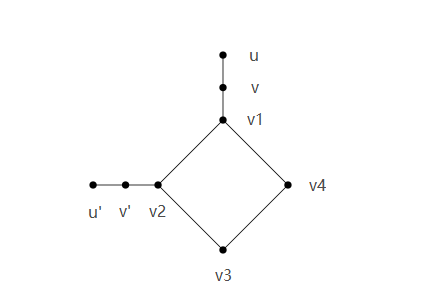
\includegraphics[width=0.5 \textwidth]{figure/notcsecuretetragram.png} 
                    \caption{not $C$-secure tetragram} %最终文档中希望显示的图片标题
                    \label{figure} %用于文内引用的标签
                \end{figure}
            \end{itemize}
        Thus, we've shown that every $C$-forbidden neighbor $u$ of $v$ is on $C$.
        
        \begin{observation}
        Each 4-face $f$ that shares an edge with $C$ has final charge at most -2$t$, where $t \in \{1, 2\}$ is the number of sinks of $f$.
        \end{observation}
        
        At least one of $C$-forbidden neighbor $u$ of $v$ is adjacent to neither $v_2$ nor $v_4$ inasmuch as $(v_1, v_2, v_3, v_4)$ is not a $C$-secure tetragram. Let $C, C_1, C_2$ be three cycles composed of $C$ and the path $v_4v_1vu$. 
        \begin{figure}[H] %H为当前位置,!htb为忽略美学标准,htbp为浮动图形
            \centering %图片居中
            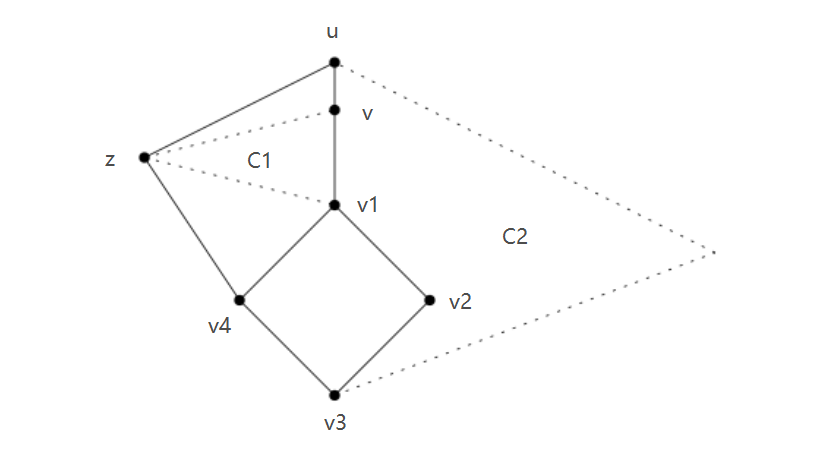
\includegraphics[width=0.8 \textwidth]{figure/cc1c2.png} 
            \caption{$C, C_1, C_2$} %最终文档中希望显示的图片标题
            \label{figure} %用于文内引用的标签
        \end{figure}
        Observed from the \textbf{Figure 34} that $v_2$ is contained in $C_2$. So from \textbf{Corollary 7.1.1.} that the length of $C_2$ is at most six. Assume that the length of $C_2$ is exactly six, it results that $v_2$ has degree three and is adjacent to $u$, which is a contradiction.\\ \\
        For this reason, the length of $C_2$ is at least seven. We conclude that the length of $C_1$ is at most 5, because the length of $C$ is at most six: $\ell_{C_1} + 7 - 2 \cdot 3 \leq 6 \Longleftrightarrow \ell_{C_1} \leq 5$. By means of the constraint of $u$, the length of $C_1$ is exactly five as in \textbf{Figure 34}. Thereby, there is exactly a vertex $z$ that is adjacent to $u$, $v_4$ and has degree two. If $z$ would have degree at least three, then it would form a triangle or against the planarity. Let $\gamma$ be the tetragram and $f(\gamma)$ be the face that is bounded by $C_1$. 
        \begin{definition}
        A tetragram $\gamma$ ($v_1, v_2, v_3, v_4$) is \textit{bad}, if $f(\gamma)$ is defined. 
        \end{definition}
        
        \begin{observation}
        Bad tetragrams are faces of $G$ that have always negative final charge. \cite{dvorak2013threecoloring}
        \end{observation}
        Assume that the number of bad tetragrams in $G$ is $b$. The initial charge of face $f(\gamma) = 9 \cdot 5 - 36 = 9$. Since 
        \begin{itemize}
            \item $v_1$ is a sink: $v_1 \notin V(C)$ and has degree three.
            \item $z \in V(C)$ and has degree two.
            \item $v \notin V(C)$ and has degree three. 
        \end{itemize}
        $f(\gamma)$ sends each three units to $u, v, v_1$ using rule (A). In addition, $f(\gamma)$ receives one unit either from $v_3$ using rule, if $v_2$ has degree exactly three; or from $v_2$ using rule (F), if $v_2$ has degree at least four so that the final charge of $f(\gamma)$ is -1. What's more, if there is another tetragram $\gamma^{'}$ that is different than $\gamma$ such that $f(\gamma) = f(\gamma^{'})$. As a result, the final charge of $f(\gamma)$ is at most $-b$.
        
        \begin{figure}[H] %H为当前位置,!htb为忽略美学标准,htbp为浮动图形
            \centering %图片居中
            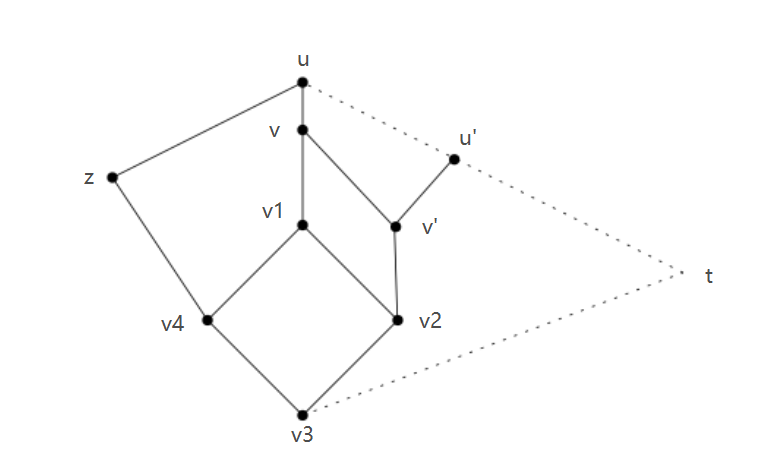
\includegraphics[width=0.7 \textwidth]{figure/temp.png} 
            \caption{$C$-secure octagram ($v, v^{'}, v_2, v_1$)} %最终文档中希望显示的图片标题
            \label{figure} %用于文内引用的标签
        \end{figure}
        Noticed that $v_3, v_4, u$ have degree at least three. From \textbf{Corollary 7.1.2.} informed that the total charge of $G$ is then at most -3, which follows $b \geq 3$. There must be another bad tetragram for $b > 1$. Hence, the final charge of $G$ is at most -4. It leads $b \geq 4$. Let $u^{'}$ be the unique neighbor of $u$ in $C \backslash z$. Noticed that $v_3v_4$ and $uu^{'}$ are the only edges of $C$ 
       incident to a bad tetragram. We conclude that $G$ has a vertex $v^{'}$ of degree three with neighbors $v, v_2, u^{'}$ and hence $v^{'}$ is a sink and $C$-admissible. And it implies that according to the definition of sink, $v_2$ is then $C$-admissible. Noticed that $u^{'}v^{'}v_2v_3t$ bounds also a face which is similar to the 5-face $zv_4v_1vu$. It follows that $(v, v^{'}, v_2, v_1)$ is a $C$-secure octagram, because $v, v^{'}, v_2, v_1$ are all $C$-admissible as proved.\\
        All in all, in any case, there will be a $C$-secure multigrams in $G$, as claimed.

    \end{itemize}
\end{itemize}
\end{proof}

